\newpage
\section{LITERATURE REVIEW}

\subsection{Human Audio Perception}

The human ear is an exceedingly complex organ.  To make matters even more difficult, the information from two ears is combined in a perplexing neural network,
the human brain. \cite{smith2013}\\
\\
\textit{Figure 1} illustrates the major structures and processes that comprise the human ear. The outer ear is composed of two parts, the visible flap of skin and
cartilage attached to the side of the head, and the ear canal, a tubeabout 0.5 cm in diameter extending about three cm into the head. These structures direct environmental
sounds to the sensitive middle and inner ear organs located safely inside of the skull bones. Stretched across the end of the ear canal is a thin sheet of tissue called the
tympanic membrane or eardrum. Sound waves striking the tympanic membrane cause it to vibrate. The middle ear is a set of small bones that transfer this vibration to the cochlea
(inner ear) where it is converted to neural impulses. The cochlea is a liquid filled tube roughly two mm in diameter and three cm in length.
\begin{figure}[h]
        \centering
        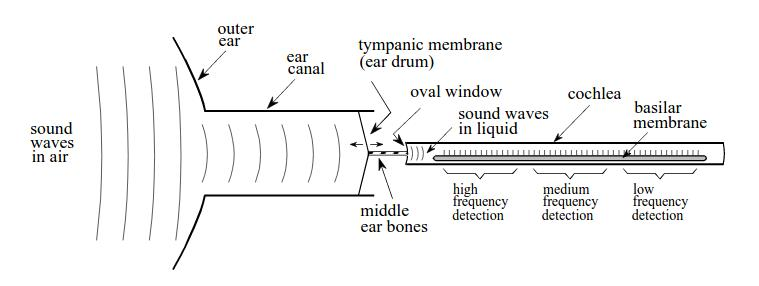
\includegraphics[width=150mm]{resources/humanear.jpg}
        \caption{Functional Diagram of Human Ear}
        \label{fig:figure1}
\end{figure}

Music can be defined as organised sound comprising the following structural elements: pitch, timbre, key, harmony, loudness (or amplitude), rhythm, meter, and tempo. Processing
these elements involves almost every region of the brain and nearly every neural subsystem.\\
\\
Sound does not exist outside of the brain; it is simply air molecules moving. Sound is produced by vibrating air molecules connecting with the
eardrum at varying frequencies (pitch) and velocities (amplitude). The process starts with the brain’s primary auditory cortex receiving a signal from the eardrum/inner ear
which immediately activates our ‘primitive’ brain, the cerebellum. The cerebellum is the oldest part of the brain in evolutionarily terms and plays an important part in motor control.
It contributes to coordination, precision, and accurate timing of movements. The ear and the primitive brain are known collectively as the low-level processing units. They perform the
main feature extraction which allows the brain to start analysing the sounds, breaking down the sensory stimulus into pitch, timbre, spatial location, amplitude, reverberant environment,
tone durations, and onset times of different notes. \\
\\
This data is conducted through neurons in the brain; cells specialized in transmitting information, and the basic building blocks of the nervous system.
The output of these neurons connects to the high-level processing units located in the frontal lobe of the brain. It is important to note that this process
is not linear. The different regions of the brain constantly update each other with new information. \\

\subsection{History of MIR and Music Classification}

The field of Music Information Retrieval (MIR) can be traced back to the 60s with reference to the works done by Kassler in \cite{kassler1966}.
Even Automatic Transcription of Music was attempted as early as the 70s \cite{andel1975}. However, there were two limiting factors that prevented progress in the field at the time.
Firstly, the high computational requirements of the problem domain was simply not available. 
And secondly, other related fields of study such as Digital Signal Processing, Speech Processing, and Machine Learning were also not advanced enough.  
So, the field stalled for the next few decades.\\
\\
In the 1990s, the field regained prominence as computational resources improved greatly and the rise of the internet resulted in massive online music collection. So, there was both an opportunity and demand for MIR systems.
The organization of the first International Symposium on Music Information Retrieval (ISMIR 1) in 2000 highlights this resurgence of interest in the field. 
280 people from 25 different countries participated in ISMIR Conference Malaga 2015.\\
\\
As for the methodologies used, MIR in the 90s was influenced by the field of Text Information Retrieval (IR), techniques for searching and retrieving text documents based on user queries.
So, most of the algorithms were developed based on symbolic representations such as MIDI files \cite{Tzanetakis2002a}. One such method is described in \cite{alghoniemy1999}.\\
\\
However, as mentioned in \cite{byrd2002}, identifying approximate units of meaning in MIR, as done by the majority of text-IR methods (words serve as such units) was not easy.\\
\\
Instead, statistical non-transcriptive approaches for non-speech audio signals started being adopted in the second half on the 90s \cite{Tzanetakis2002a}.
This was probably influenced by progress of such methods in other fields of speech processing. 
For example, in \cite{saunders1996}, the authors reported 98 per cent accuracy in distinguishing music from speech in commercial radio broadcasts.
This was based on the statistics of the energy contour and the zero-crossing rate.\\
\\
In \cite{wold1996}, the authors introduced similar statistical methods for retrieval and classification of isolated sounds.
Similarly, in \cite{scheirer1997}, an algorithm for music-speech classification based on spectral feature was introduced. 
It was trained using supervised learning. \\
\\
And so, starting in the 2000s, instead of methods attempting note-level transcriptions, researchers focused on direct extraction of information of audio signals using Signal Processing and Machine Learning techniques.\\
\\
Currently, three basic strategies are being applied in MIR: \cite{Casey2008}

\begin{itemize}
        \item \textbf{Based on Conceptual Metadata} - Suited for low-specificity queries.

        \item \textbf{Using High-level Descriptions} - Suited for mid-specificity queries.

        \item \textbf{Using Low-level Signal-based Properties} - Used for all specificities.

\end{itemize}

But still most of the MIR techniques being employed at present use low-level signal features instead of high-level descriptors \cite{Kaminskas2012}.
Thus, there exists a semantic gap between human perception of music and how MIR systems work.

\subsection{Audio Processing}

General Audio signal processing is an engineering field that focuses on the computational methods for intentionally altering sounds, methods that
are used in many musical applications.\\
\\
Particularly speaking, music signal processing may appear to be the junior relation of the large and mature field of speech signal processing,
not least because many techniques and representations originally developed for speech have been applied to music, often with good results. However,
music signals possess specific acoustic and structural characteristics that distinguish them from spoken language or other nonmusical signals. \cite{muller2011}\\
\\
In music the most important qualities of sound are: pitch, duration, loudness, and timbre. Duration and loudness are unidimensional, while pitch and timbre are complex and multidimensional. \cite{dooling2014}

\begin{itemize}
        \item \textbf{Loudness} - Intensity of a tone is the physical correlate that underlies the perception of loudness. Loudness variations play an important role in music, but are less important than pitch variations.

        \item \textbf{Duration} - A composer or performer can alter the pace of a piece so that its apparent (virtual) time is slower or faster than clock time. 

        \item \textbf{Timbre} - Timbre is the subjective code of the sound source or of its meaning. According to the American Standards Association, "Timbre
                is that attribute of auditory senstation of which a listener can judge that two steady-state tones having the same pitch and loudness are dissimilar."

        \item \textbf{Pitch} - Pitch is related to the frequency of a pure tone and to the fundamental frequency of a complex tone. In its musical sense, pitch
                has a range of about 20 to 5000 Hz. Some five to Zseven harmonics of a complex tone can be heard out individually by paying close attention. There
                is a dominance region for pitch perception, roughly from 500 to 2000 or 3000 Hz. Harmonics falling in the dominance region are most influential 
                with regard to pitch.

\end{itemize}

Again, these types of low dimensional features extracted from the acoustical signals are more popular than higher dimensional representations such as
Spectrograms for Classification purposes. \cite{prasad2007}

\subsection{Related Works}
\subsubsection{Genre Based Classification}

\paragraph{Overview.}
Automatic Music Genre Classification (AMGC) is one of the tasks focused by MIR. However, it is not a straightforward one.\\
\\
In \cite{Scaringella2006}, Scaringella et al. discuss how and why musical genres are a poorly defined concept making the task of automatic classification non-trivial.
Still, although the boundaries between genres are fuzzy and there are no well-defined definitions, it is still one of the widely used method of classification of music. 
If we look at human capability in genre classification, Perrot et al \cite{Perrot1999} found that people classified songs--in a ten-way classification setup--with an accuracy of 70 per cent after listening to 3s excerpts.

\paragraph{Features.}
The features used for genre based classification have been heavily influenced by the related field of speech recognition. 
For instance, Mel-frequency Cepstral Coefficients (MFCC), a set of perceptually motivated features that is widely used in music classification, was first used in speech recognition.\\
\\
The seminal paper on musical genre classification by Tzanetakis et al. \cite{Tzanetakis2002} presented three feature sets for representing timbral texture, rhythmic content and pitch content. 
With the proposed feature set, they achieved a classification accuracy of 61 per cent for ten musical genre.\\
\\
Timbral features are usually calculated for every short-time frame of sound based on the Short Time Fourier Transform (STFT). 
So, these are low-level features. 
Typical examples are Spectral Centroid, Spectral Rolloff, Spectral Flux, Energy, Zero Crossings, and the afore-mentioned Mel-Frequency Cepstral Coefficients (MFCCs).
Among these, MFCC is the most widely preferred feature \cite{Lippens2004}\cite{Kour2015}. Logan \cite{Logan2000} investigated the applicability of MFCCs to music modeling and found it to be "at least not harmful".\\
\\
Rhythmic features capture the recurring pattern of tension and release in music while pitch is the perceived fundamental frequency of the sound. 
These are usually termed as mid-level features.\\
\\
Apart from these, many non-standard features have been proposed in the literature. \\
\\
Li et al.\cite{Li2003} proposed a new set of features based on Daubechies Wavelet Coefficient Histograms (DWCH), and also presented a comparative study with the features included in the MARSYAS framework.
They showed that it significantly increased the accuracy of the classifier.\\
\\
Anglade, Amélie, et al.\cite{Anglade2010} propose the use of Harmony as a high-level descriptor of music, focusing on the structure, progression, and relation of chords.\\
\\

\paragraph{Classifer.}

A variety of methods have been used for music classification. Some of the popular ones are SVM, K Nearest Neighbours and variants of Neural Networks.
The results are also widely different. In \cite{Neumayer2004}, 61 per cent accuracy has been achieved using a Multilayer Perceptron based approach. 
While in \cite{Koerich2013}, the authors have achieved 71 per cent accuracy through the use of an additional rejection and verification stage.
Haggblade et al. \cite{Haggblade2011}, compared simpler and more naive approaches (k-NN and k-Means) with more sophisticated neural networks and SVMs. 
They found that the latter gave better results.\\
\\
Standard statistical pattern recognition classifiers are also used for AMGC.
They may be simple Gaussian Classifiers or Gaussian mixture model (GMM) classifier, where each class pdf is assumed to consist of a mixture of a specific number of multidimensional Gaussian distributions.
In such an approach, the parameters of each Gaussian component and the mixture weights are estimated using the iterative EM algorithm.\\
\\
However, lots of unique methods -- either completely novel or a variation of a standard method -- have been put into use too. In \cite{Nasridinov2014}, the authors
propose a method that uses Chord labeling (ones and zeros) in conjunction with a k-windowSubsequenceMatching algorithm used to find subsequence in music sequence
and a Decision tree for the actual genre classification.\\
\\
It is also noted that high-level and contextual concepts can be as important as low-level content descriptors. \cite{Anglade2010} 

\subsubsection{Mood Based Classification}

\paragraph{Overview.}

As mood is a very human thing, Mood Based Classification, also known as Mood Emotion Recognition (MER), requires knowledge of both technical aspects as well as the human emotional system.
So, the conceptualization of emotion and understanding of the associated emotion taxonomy is vital. However, it is a difficult thing to do, because 
\begin{enumerate}[(i)]
        \item It is subjective and 

        \item We cannot agree on a model to depict emotional states.
        \end{enumerate}

Usually, two approaces to emotion conceptualization are taken: 

\begin{itemize}
    \item \textbf{Categorical Conceptualization} - This approach to MER categorizes emotions into a number of distinct classes. 
        It requires the belief of base emotions (happiness, anger, sadness, etc) from which all other secondary emotion classes can be derived.\cite{Ekman1992}
        However, the major drawback of the categorical approach is that the number of primary emotion classes is too small in comparison with the richness of music emotion perceived by humans.

    \item \textbf{Dimensional Conceptualization} - It defines Musical Values as numerical values over a number of emotion dimensions. 
        So, the focus is on distinguishing emotions based on their position on a predefined space.
        Most of these conceptualizations map to three axes of emotions: valence (pleasantness), arousal (activation) and potency (dominance).
        By placing emotions on a continuum instead of trying to label them as discrete, this approach can encompass a wide variety of general emotions.

\end{itemize}

\paragraph{Circumplex and Thayer Mood Model.}

One of the Dimensional conceptualization was proposed by Russell (1980) \cite{Russell1980}.
As shown in \textit{Figure 2}, the model consists of a two-dimensional structure involving the dimensions of valence and arousal. 
General emotions are placed within thic circular framework.

\begin{figure}[hlvt!]
        \centering
        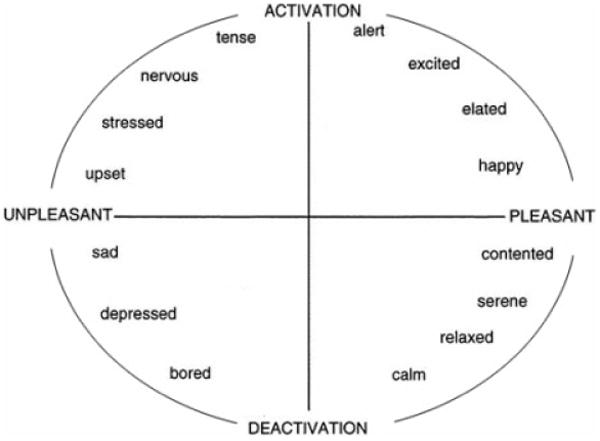
\includegraphics[width=120mm]{resources/circumplex.jpg}
        \caption{A graphical representation of the circumplex model of affect with the horizontal axis representing the valence dimension and the vertical axis representing the arousal or activation dimension.}
        \label{fig:figure2}
\end{figure}

As shown in \textit{Figure 3}, Thayer \cite{Thayer1990} proposed a similar two-dimensional approach that adopts the theory that mood is entailed from two factors: -Stress (happy/anxious) -Energy (calm/ energetic). 
This divides music mood into four clusters: Contentment, Depression, Exuberance and Anxious/Frantic.\\
\\
Although, the two-dimensional approach has been criticized as deficient (leading to a proposal of the third dimension of potency), it seems to offer the right balance between sufficient "verbosity" and low complexity \cite{Juslin2001}.

\begin{figure}[hlvt!]
        \centering
        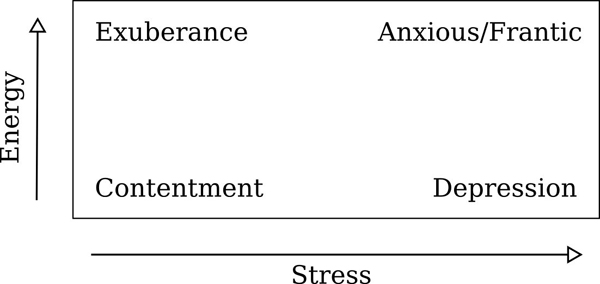
\includegraphics[width=120mm]{resources/thayerModel.jpg}
        \caption{Thayer's two-dimensional model of mood}
        \label{fig:figure3}
\end{figure}

\paragraph{Features.}

Some of the commonly used features in MER are:

\begin{itemize}
    \item \textbf{Energy}: Energy related features such as audio power, loudness, specific loudness sensation coefficients (SONE), are correlated to the perception of arousal. 
        Lu et al. \cite{Lu2006} used it to classify arousal.

    \item \textbf{Rhythm}: Flowing/fluent rhythm is associated with positive valence while firm rhythms with negative valence.

    \item \textbf{Melody}: These include features such as Pitch (perceived fundamental frequency), chromogram centroid, etc.

    \item \textbf{Timbre}: As with the AMGC problem, MFCC is widely used in MER too. Apart from MFCC, octave-based spectral contrast as well as DWCH (Daubechies wavelets coefficient histogram) are also proposed in literature.
        
\end{itemize}

So, we see that the features used in MER are almost the same as those in AMGC. However, Fu et al. note in their extensive survey on Audio-based Music Classification \cite{Fu2011} that although their effectiveness is debatable, mid-level features such as Rhythm seem to be more popular in MER.


\paragraph{Classifiers.}

The algorithms used in AMGC are also popular in MER. So, support vector machines, Gaussian mixture models, neural networks, and k-nearest neighbor are the ones regularly used.

